% !TEX root = ../main.tex

\chapter{Evaluation}\label{chap:evaluation}

After the proposed methodology was implemented, a dedicated evaluation protocol was devised to evaluate the proposed model in comparison to a state-of-the-art parametric  \ac{TTS} system.
In this chapter, I describe how the stimuli for the evaluation were prepared, the evaluation protocol, the results of the evaluation, and a discussion.

\section{Stimuli Preparation}

To run the evaluation, the 2017 Blizzard Challenge\footnote{For details on the Blizzard Challenge see \url{https://synsig.org/index.php/Blizzard_Challenge_2017}} speech corpus\footnote{The corpus, originally made available by Usborne publishing (\url{https://usborne.com/}), is available at \url{http://www.cstr.ed.ac.uk/projects/blizzard/2017/usborne_blizzard2017/}} was used.
The full corpus comprises about 6.5 hours of speech taken from a number of children's audiobooks, all read by a British female speaker.

The corpus was automatically aligned and pre-processed with the Montreal Forced Aligner \citep{McAuliffe2017Montreal} and the MaryTTS system \citep{LeMaguer2017Uprooting}, producing 3866 utterances for a total of 3~h and 57~min of speech.
The corpus was then split into three subsets: a training set (3475 utterances), a validation set (211 utterances), and a test set (180 utterances).

For the evaluation, three sources of intonation were considered: the intonation estimated from the original recording, the intonation produced with the proposed methodology, and finally, the intonation produced by the Merlin toolkit\footnote{The implementation of the Merlin toolkit is available at: \url{https://github.com/CSTR-Edinburgh/merlin}} \citep{Wu2016Merlin}.
The Merlin toolkit makes for a particularly apt comparison, because it also uses \ac{DNN} technology, albeit in a very different way, as intonation and other acoustic features are modeled jointly.

As the main objective was to evaluate intonation, all stimuli used in the evaluation protocol were first neutralized with respect to duration and spectral features, to ensure that stimuli produced by different systems are comparable with respect to their intonation.

Duration was neutralized by imposing the duration of the original recordings extracted during the forced-alignment step.
As for the neutralization of the spectral features, it was not possible to use the acoustic features extracted from the original recordings:
even though vocoders based on the source-filter model can theoretically separate the periodic information from the spectral features and the aperiodic features, in reality vocoders often do not achieve perfect decorrelation of these sets of features.
As consequence, replacing the estimated \ac{F0} of a recording with an arbitrary one will most likely result in substantial quality degradation.

In order to inhibit the effects of the spectrum, a \ac{DNN} segmental synthesizer was implemented.
The segmental synthesizer used for the stimuli preparation is described in detail in \autoref{chap:segmental-synthesizer}.
For the training of the segmental synthesizer, the same training, test, and validation sets were used.
The \ac{MCD}
of the synthesizer measured on the test set was around 7~dB.


\section{Evaluation protocol}

As currently no objective evaluation can reliably assess the quality of the intonation of speech, a dedicated evaluation protocol based on subjective evaluation was devised.
Subjective evaluations are primarily designed to probe more subjective and intangible aspects of speech that cannot easily be tested by means of objective evaluation, such as intelligibility and naturalness.

The dedicated protocol for the evaluation is a classic preference AB test, i.e., subjects are exposed to a pair of stimuli and they are required to express their preference.
This choice is justified by the need to avoid the ceiling effect, as well as the lack of reproducibility and interpretability that often affects evaluations based on absolute judgments such as \ac{MOS}.
The AB preference task was also chosen for its simplicity.
As the test would be delivered online to people who might have never participated in speech evaluations, more common but also slightly more complicated evaluation protocols such as the \ac{MUSHRA} test were deemed unsuitable.

A no-preference option was not included, lest subjects should abuse this option as a way to avoid expressing strong opinions.
In order to prevent this from happening, during the evaluation, participants are always forced to make a decision.
Later on, a lack of preference can be inferred by simply looking at preference distributions.
For instance, if participants expressed preference for a system over another system within a certain percentage range, say 40\%--60\%, then we can assume there is no preference.

The evaluation was automatically prepared and managed by the online platform PercEval.\footnote{The platform was made available courtesy of the EXPRESSION group at IRISA, \url{https://www-expression.irisa.fr/}.}
The platform makes sure that stimuli are properly shuffled and spread out across participants in a statistically balanced way, so that all participants are exposed to as wide a variety of stimuli as possible and that, on average, all stimuli are seen a similar number of times.

From the test corpus, 180 distinct pairs were constructed.
After providing the pairs and a set of configuration parameters, the platform started generating experiments on-demand.
Whenever a new participant was available, a new experiment was generated and delivered online.

At the start of the evaluation, each participant was required to provide an email address and to take the brief questionnaire shown in \autoref{fig:questionnaire}.

\begin{figure}[H]
\centering
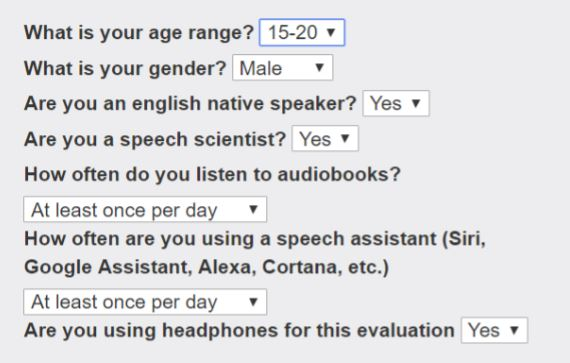
\includegraphics[scale=.5]{figures/questionnaire.png}
\caption[Evaluation questionnaire]{Questionnaire displayed before the evaluation.}
\label{fig:questionnaire}
\end{figure}

After the questionnaire, participants were introduced to a quick simulation, in which 6 of the total 180 pairs were used to allow them to familiarize themselves with the evaluation environment.

Of the 174 remaining pairs, each participant listened to 60 pairs, each selected randomly using a balanced random selection algorithm.
At each step of the evaluation (here shown in \autoref{fig:eval-step}), subjects were presented with a pair of stimuli, a transcription of the corresponding text, as well as the question: ``Which way of reading the following text do you prefer, A or B?''


\begin{figure}[H]
\centering
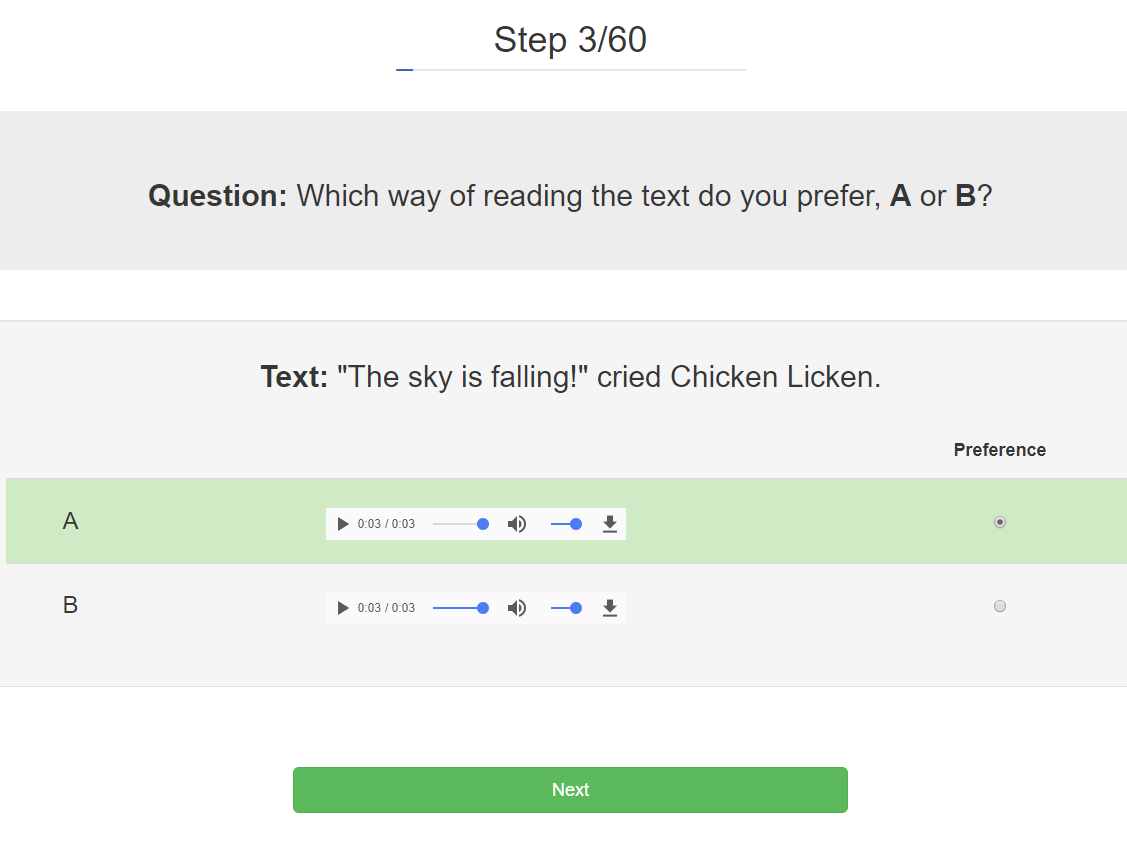
\includegraphics[scale=.4]{figures/evaluation-environment.png}
\caption[Evaluation step]{Screenshot of one evaluation step.}
\label{fig:eval-step}
\end{figure}

\clearpage

\section{Results and Discussion}


In total, 40 listeners participated in the evaluation. 
Of these, 10 were native speakers of English.
The results of their evaluation are  shown in \autoref{fig:eval-results} (for more details on the results, see \autoref{sec:appendix-d}).

\begin{figure}[H]
\centering
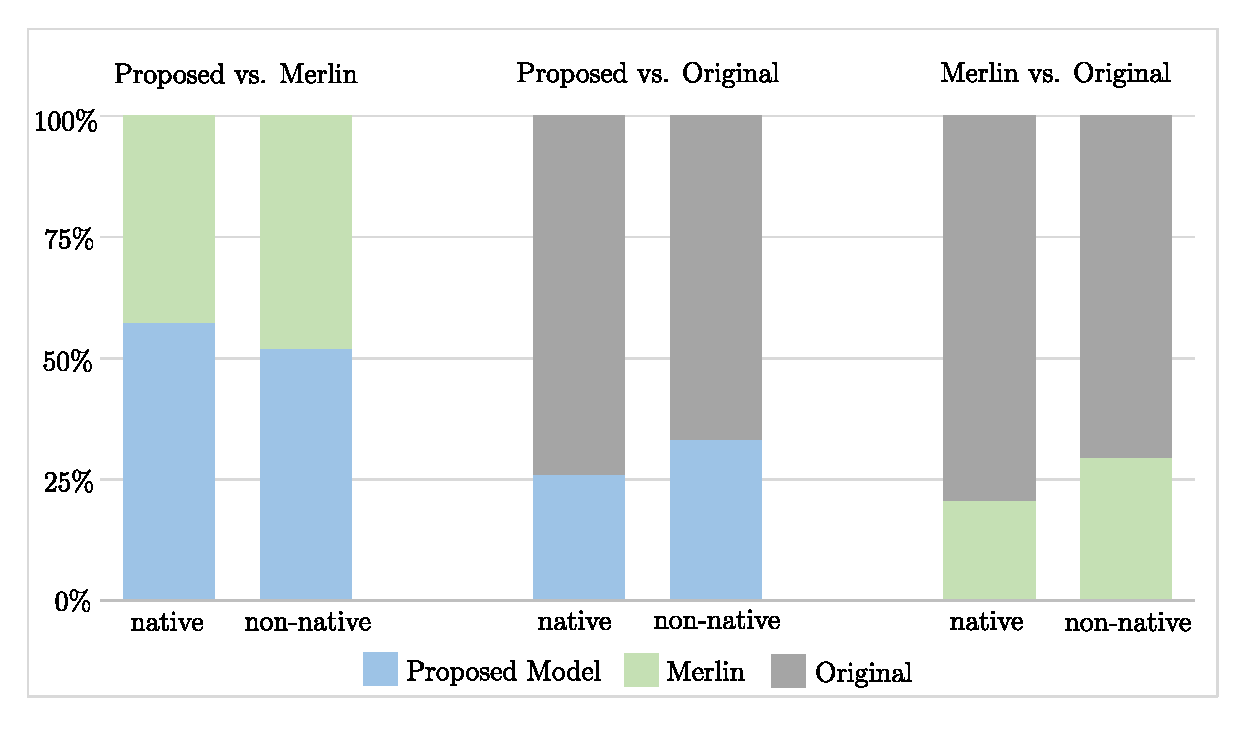
\includegraphics[scale=.5]{figures/eval-chart.pdf}
\caption[Evaluation results]{Preference evaluation results.}
\label{fig:eval-results}
\end{figure}

The most noticeable trend is the clear preference of both native and non-native subjects for the natural intonation over the automatically generated ones.
This trend is amplified for the native subjects, where preference for the natural intonation can reach as high as 79.4\% (Merlin vs.\ Original).

Comparing the proposed model to Merlin, the two seem to be more or less equivalent for the non-native listeners (52.0\% vs.\ 48.0\%).
However, if we look at the results for the native subjects, there seems to be a slight preference for the proposed model (57.4\% vs.\ 42.6\%).

Overall, these results do not show a very strong preference for either system.
However, the difference between the results of the native and non-native subjects is not negligible and might imply that the proposed model is able to capture more specific phenomena, which are going undetected by the non-native subjects.
What the nature of these phenomena might be is unclear, but their effect is strong enough to warrant further investigation.

Because the evaluation protocol was designed to be very simple, it also has limitations.
For instance, participants had to select their preference without any context.
This can be problematic for intonation evaluations, as the same intonation pattern might be correct or incorrect, depending on the context in which it is used.
However, the strong preference for the original shows that subjects were still able to distinguish the systems, even without context.

The evaluation protocol is also limited in its ability to provide more qualitative analysis of the differences between systems.
This points to a clear need for a more refined analysis protocol in order to qualify how the proposed model differs from that of Merlin.

